\chapter{Lezione 9}
\label{chap:lezione_09} 

\begin{flushright}
\textit{Data: 29/10/2025}
\end{flushright}


\section{Transitività e Coefficiente di Clustering}
Una proprietà importante delle reti è la \textbf{transitività}, espressa colloquialmente per le reti sociali come: "l'amico del mio amico è mio amico". Questo concetto misura la tendenza dei nodi a formare triangoli (triadi).

\begin{itemize}
\item \textbf{Transitività Perfetta:} Si verifica nelle \textbf{cliques} (o cricche), che sono sottografi in cui tutti i nodi sono completamente connessi tra loro (es. una 3-clique è un triangolo).
\item \textbf{Transitività Parziale:} Il caso più generale in cui un amico di un amico non è necessariamente un amico.
\end{itemize}

Questa proprietà è quantificata dal \textbf{Coefficiente di Clustering ($C$)}.

\subsection{Coefficiente di Clustering Globale}
Il coefficiente di clustering globale $C$ è una misura riferita all'intera rete. È definito come la frazione di "triadi aperte" (cammini di lunghezza 2) che sono "chiuse" (ovvero, formano un triangolo).

\begin{equation}
C = \frac{\text{\# di cammini chiusi di lunghezza 2}}{\text{\# di cammini di lunghezza 2}}
\end{equation}
Alternativamente, poiché ogni triangolo contiene 6 cammini chiusi di lunghezza 2 (ad es., $1\to2\to3$, $1\to3\to2$, $2\to1\to3$, ecc.), questo può essere scritto come:

\begin{equation}
C = \frac{\text{\# di triangoli} \times 6}{\text{\# di cammini di lunghezza 2}}
\end{equation}

\begin{center}
\begin{tikzpicture}[scale=0.5]
    \tikzset{
        simple_node/.style={
            text=black
        },
        black_edge/.style={
            line width=1.5pt,
            colorB
        },
        red_dotted/.style={
            color=colorE,
            line width=2pt,
            loosely dotted, % Punti distanziati
            line cap=round  % Punti rotondi
        }
    }

    % Posizionamento nodi
    \node[simple_node] (2) at (0, -1) {2};       % Nodo sinistro
    \node[simple_node] (1) at (3, 2) {1};       % Nodo in alto
    \node[simple_node] (3) at (4.5, -0.8) {3};  % Nodo intermedio destro
    \node[simple_node] (4) at (4, -2.5) {4};    % Nodo in basso

    % Archi neri solidi
    \draw[black_edge] (2) -- (1);
    \draw[black_edge] (2) -- (3);
    \draw[black_edge] (2) -- (4);
    \draw[black_edge] (3) -- (4);

    % Linea rossa tratteggiata tra 1 e 3 (o tra 1 e il gruppo in basso)
    \draw[red_dotted] (1) -- (4);
    \draw[red_dotted] (1) -- (3);


\end{tikzpicture}
\end{center}

\subsubsection{Esempi}
\begin{enumerate}
\item Triangolo Completamente Connesso (3-clique):
I cammini di lunghezza 2 sono: $1\to2\to3$, $1\to3\to2$, $2\to1\to3$, $2\to3\to1$, $3\to1\to2$, $3\to2\to1$.
\begin{itemize}
\item \# di cammini di lunghezza 2 = 6.
\item Tutti e 6 questi cammini sono chiusi (es. per $1\to2\to3$, esiste il collegamento $1-3$).
\item $C = \frac{6}{6} = 1$.
\end{itemize}

\item Grafo a 4 Nodi (Triangolo + 1 nodo):
Consideriamo i nodi $\{i, j, k, l\}$, dove $\{i, k, l\}$ formano un triangolo, e $j$ è connesso solo a $i$.
% FIGURE PLACEHOLDER: Un grafo a triangolo (i, k, l) con un nodo extra (j) attaccato solo al nodo i
I cammini di lunghezza 2 sono:
\begin{itemize}
\item Da $j$: $j \to i \to k$, $j \to i \to l$ (2 cammini)
\item Da $k$: $k \to i \to j$, $k \to i \to l$, $k \to l \to i$ (3 cammini)
\item Da $l$: $l \to i \to j$, $l \to i \to k$, $l \to k \to i$ (3 cammini)
\item Da $i$: $i \to k \to l$, $i \to l \to k$ (2 cammini)
\end{itemize}
\begin{itemize}
\item Numero totale di cammini di lunghezza 2: $2+3+3+2 = 10$.
\item Solo i cammini all'interno del triangolo $\{i, k, l\}$ sono chiusi. Questi sono i 6 cammini dell'Esempio 1 (es. $i \to k \to l$ è chiuso da $i-l$, $k \to i \to l$ è chiuso da $k-l$, ecc.).
\item $C = \frac{6}{10} = \frac{3}{5}$.
\end{itemize}
\end{enumerate}

\subsubsection{Valori Empirici}
Le reti del mondo reale tendono ad avere alti coefficienti di clustering, ben lontani da quanto previsto in un grafo casuale semplice.
\begin{itemize}
\item Collaborazioni attori cinematografici: $C \approx 0.20$
\item Collaborazioni biologi: $C \approx 0.09$
\item Reti di email: $C \approx 0.16$
\end{itemize}
In un grafo casuale semplice e grande con $n$ nodi e grado medio $\langle k \rangle$, la probabilità che due nodi qualsiasi siano connessi è $p = \langle k \rangle / (n-1)$. La probabilità che due amici di un nodo siano anche amici tra loro è questa stessa $p$.
Pertanto, per un grafo casuale $C \approx p = \frac{\langle k \rangle}{n-1}$. Per $n \to \infty$, $C \to 0$. Ciò dimostra che i grafi casuali non sono buoni modelli per l'alto clustering osservato nelle reti reali.

\subsection{Coefficiente di Clustering Locale}
Possiamo definire anche un coefficiente di clustering $C_i$ per un singolo nodo $i$.
\begin{equation}
C_i = \frac{\text{\# di coppie di vicini di } i \text{ che sono connesse}}{\text{\# di coppie di vicini di } i}
\end{equation}
Il denominatore è il numero totale di possibili triangoli centrati in $i$, che è il numero di modi per scegliere 2 vicini tra $k_i$, ovvero $\binom{k_i}{2} = \frac{k_i(k_i-1)}{2}$.

\noindent Il numeratore è il numero di triangoli che esistono effettivamente coinvolgendo il nodo $i$. Questo può essere trovato usando la matrice di adiacenza. Un triangolo $i-j-k-i$ esiste se $A_{ij}=1$, $A_{jk}=1$, e $A_{ki}=1$. Il numero di triangoli connessi a $i$ è $\frac{1}{2}\sum_{j,k} A_{ij} A_{jk} A_{ki}$. Il fattore $\frac{1}{2}$ è presente perché la somma conta $i\to j\to k\to i$ e $i\to k\to j\to i$ come distinti.

\noindent Il coefficiente di clustering locale è:
\begin{equation}
C_i = \frac{\frac{1}{2}\sum_{j,k} A_{ij} A_{jk} A_{ki}}{\frac{1}{2}k_i(k_i-1)} = \frac{\sum_{j,k} A_{ij} A_{jk} A_{ki}}{k_i(k_i-1)}
\end{equation}

\noindent Il coefficiente di clustering globale $C$ può quindi essere definito come la media dei $C_i$ locali, pesata dal numero di possibili triangoli per ogni nodo:
\begin{equation}
C = \frac{\sum_i C_i \binom{k_i}{2}}{\sum_i \binom{k_i}{2}} = \frac{\sum_i \left( \frac{\sum_{j,k} A_{ij} A_{jk} A_{ki}}{k_i(k_i-1)} \right) \frac{k_i(k_i-1)}{2}}{\sum_i \frac{k_i(k_i-1)}{2}} = \frac{\sum_{i,j,k} A_{ij} A_{jk} A_{ki}}{\sum_i k_i(k_i-1)}
\end{equation}
Questa formula mostra che $C$ è calcolabile semplicemente dalla matrice di adiacenza $A$ (poiché $k_i = \sum_j A_{ij}$).

\section{Assortatività}
L'assortatività descrive la tendenza dei nodi a connettersi ad altri nodi che sono simili a loro. La "similitudine" può essere definita sulla base di varie caratteristiche.
\begin{itemize}
\item \textbf{Grado:} Questa è la più comune.
\begin{itemize}
\item \textbf{Assortativa:} Nodi ad alto grado si connettono a nodi ad alto grado (es. reti sociali).
\item \textbf{Disassortativa:} Nodi ad alto grado (hub) si connettono a nodi a basso grado (es. reti tecnologiche come Internet, o reti di interazione proteica).
\end{itemize}
\item \textbf{Caratteristiche non ordinate:} Nazionalità, genere, razza.
\item \textbf{Caratteristiche ordinate:} Età, reddito.
\end{itemize}

L'assortatività è una correlazione, quindi la misuriamo usando la covarianza. Sia $x_i$ il valore di una caratteristica per il nodo $i$. Il valore atteso $\mu$ di questa caratteristica, mediato sugli estremi di tutti i collegamenti, è:
\begin{equation}
\mu = \frac{1}{2m} \sum_i k_i x_i
\end{equation}
dove $2m = \sum_i k_i = \sum_{ij} A_{ij}$ è la somma di tutti i gradi.

\noindent La covarianza per questa caratteristica attraverso tutte le coppie di nodi connessi è:
\begin{equation}
\text{cov}(x, x') = \frac{1}{2m} \sum_{i,j} A_{ij} (x_i - \mu)(x_j - \mu)
\end{equation}
Il termine $A_{ij}$ assicura che sommiamo solo sui nodi connessi $i$ e $j$.

\subsection{Assortatività per Grado}
Analizziamo il caso specifico in cui la caratteristica è il grado stesso, $x_i = k_i$.
Il valore atteso $\mu$ diventa:
\begin{equation}
 \mu = \frac{1}{2m} \sum_i k_i (k_i) = \frac{1}{2m} \sum_i k_i^2
\end{equation}

\noindent Calcoliamo la covarianza.
\begin{align*}
\text{cov}(k, k') &= \frac{1}{2m} \sum_{i,j} A_{ij} (k_i - \mu)(k_j - \mu) \\
&= \frac{1}{2m} \sum_{i,j} A_{ij} (k_i k_j - \mu k_i - \mu k_j + \mu^2) \\
&= \frac{1}{2m} \left[ \sum_{i,j} A_{ij} k_i k_j - \mu \sum_{i,j} A_{ij} k_i - \mu \sum_{i,j} A_{ij} k_j + \mu^2 \sum_{i,j} A_{ij} \right]
\end{align*}
Semplifichiamo i termini:
\begin{itemize}
\item $\sum_{i,j} A_{ij} k_i = \sum_i k_i \left( \sum_j A_{ij} \right) = \sum_i k_i (k_i) = \sum_i k_i^2$
\item $\sum_{i,j} A_{ij} k_j = \sum_j k_j \left( \sum_i A_{ij} \right) = \sum_j k_j (k_j) = \sum_j k_j^2$
\item $\sum_{i,j} A_{ij} = 2m$
\end{itemize}
Sostituiamo questi termini:
\begin{align*}
\text{cov}(k, k') &= \frac{1}{2m} \left[ \sum_{i,j} A_{ij} k_i k_j - \mu \sum_i k_i^2 - \mu \sum_j k_j^2 + 2m \mu^2 \right] \\
\text{Usando } \sum_i &k_i^2 = 2m \mu \text{ (dalla def. di } \mu \text{)} \\
&= \frac{1}{2m} \left[ \sum_{i,j} A_{ij} k_i k_j - \mu (2m \mu) - \mu (2m \mu) + 2m \mu^2 \right] \\
&= \frac{1}{2m} \sum_{i,j} A_{ij} k_i k_j - \mu^2 - \mu^2 + \mu^2 \\
&= \frac{1}{2m} \sum_{i,j} A_{ij} k_i k_j - \mu^2
\end{align*}
Questa espressione può essere riscritta come:
\begin{equation}
 \text{cov}(k, k') = \frac{1}{2m} \sum_{i,j} \left( A_{ij} - \frac{k_i k_j}{2m} \right) k_i k_j
\end{equation}

Per ottenere un \textbf{coefficiente di assortatività $r$} normalizzato (correlazione di Pearson), dividiamo la covarianza per la massima covarianza possibile (la varianza):
\begin{equation}
r = \frac{\sum_{ij} (A_{ij} - \frac{k_i k_j}{2m}) k_i k_j}{\sum_{ij} (k_i \delta_{ij} - \frac{k_i k_j}{2m}) k_i k_j}
\end{equation}
Questo valore $r$ è limitato: $-1 \le r \le 1$.
\begin{itemize}
\item $r > 0$: Assortativo
\item $r < 0$: Disassortativo
\item $r = 0$: Non-assortativo
\end{itemize}
Questa formula è computazionalmente costosa ($O(n^2)$). Una formula equivalente più veloce ($O(m)$) è:
\begin{tcolorbox} [colback=yellow!25, colframe=yellow!75!orange, coltitle=black, title=\textbf{Coefficiente di Assortatività}]
\begin{equation}
r = \frac{S_1 S_e - S_2^2}{S_1 S_3 - S_2^2}
\end{equation}
dove $S_n = \sum_i k_i^n$ e $S_e = \sum_{ij} A_{ij} k_i k_j = 2 \sum_{\text{edges } i-j} k_i k_j$.
\end{tcolorbox}

\section{Modelli di Rete I: Grafi Casuali}
Passiamo ora ai modelli per generare reti. Il primo e più semplice è il grafo casuale, come definito da Erdős e Rényi. Ci concentreremo sul modello $G(n,p)$.

\begin{itemize}
\item \textbf{Ensemble $G(n,p)$:} Un insieme di grafi con $n$ nodi.
\item \textbf{Processo:} Per ogni possibile coppia di nodi, viene tracciato un arco con una probabilità fissa $p$.
\end{itemize}

\subsubsection{Proprietà di $G(n,p)$}
\begin{itemize}
\item \textbf{Numero Medio di Link $\langle m \rangle$:} Il numero di possibili coppie è $\binom{n}{2}$.
\begin{equation}
 \langle m \rangle = \binom{n}{2} p = \frac{n(n-1)}{2} p
 \end{equation}

\item \textbf{Grado Medio $\langle k \rangle$:} Il grado medio è $\langle k \rangle = \frac{2\langle m \rangle}{n}$.
\begin{equation}
 \langle k \rangle = \frac{2}{n} \left( \frac{n(n-1)}{2} p \right) = (n-1)p
 \end{equation}
\end{itemize}

\subsection{Distribuzione di Grado $p_k$}
La distribuzione di grado $p_k$ (la probabilità che un nodo abbia grado $k$) segue una \textbf{distribuzione binomiale}. Per un dato nodo, ci sono $n-1$ altri nodi a cui esso può connettersi.
\begin{equation}
p_k = \binom{n-1}{k} p^k (1-p)^{n-1-k}
\end{equation}
Per $n$ grande e $p$ piccolo (tale che $\langle k \rangle = (n-1)p$ rimanga finito), questa distribuzione binomiale converge a una \textbf{distribuzione di Poisson}.



\subsubsection{Derivazione: Da Binomiale a Poisson}
Vogliamo mostrare che $p_k \to \frac{\langle k \rangle^k e^{-\langle k \rangle}}{k!}$ quando $n \to \infty$.

\noindent Partiamo da $p_k = \frac{(n-1)!}{k!(n-1-k)!} p^k (1-p)^{n-1-k}$.

\begin{enumerate}
    \item Approssimiamo il coefficiente binomiale:
$$ \binom{n-1}{k} = \frac{(n-1)(n-2)\dots(n-k)}{k!} $$
Per $n \gg k$, ogni termine al numeratore è approssimativamente $n-1$.
$$ \binom{n-1}{k} \approx \frac{(n-1)^k}{k!} $$
\item Approssimiamo i termini di probabilità:
$$ p^k = \left( \frac{\langle k \rangle}{n-1} \right)^k = \frac{\langle k \rangle^k}{(n-1)^k} $$
$$ (1-p)^{n-1-k} = \left( 1 - \frac{\langle k \rangle}{n-1} \right)^{n-1-k} $$
Usando il limite $\lim_{x\to\infty} (1 - c/x)^x = e^{-c}$, e notando che $n-1-k \approx n-1$:
$$ (1-p)^{n-1-k} \approx \exp\left(-\langle k \rangle\right) $$
\item Combiniamo:
$$ p_k \approx \left( \frac{(n-1)^k}{k!} \right) \left( \frac{\langle k \rangle^k}{(n-1)^k} \right) \left( e^{-\langle k \rangle} \right) = \frac{\langle k \rangle^k e^{-\langle k \rangle}}{k!} $$
\end{enumerate}
 


\begin{tcolorbox}[colback=colorB!25,colframe=colorB!75!colorA,title={Distribuzione di Grado di G(n,p)}]
\begin{equation} \label{eq:poisson}
p_k = \frac{\langle k \rangle^k e^{-\langle k \rangle}}{k!}
\end{equation}
\end{tcolorbox}

Questa distribuzione ha un picco attorno a $\langle k \rangle$. Tutti i nodi sono statisticamente simili. Questo è un grafo "democratico", ma non riproduce gli "hub" (leggi di potenza) osservati in molte reti reali.

\subsubsection{Coefficiente di Clustering di $G(n,p)$}
Il coefficiente di clustering è la probabilità che due vicini di un nodo siano anche vicini tra loro. In $G(n,p)$, la probabilità che due nodi qualsiasi siano connessi è $p$.
\begin{equation}
 C = p = \frac{\langle k \rangle}{n-1}
\end{equation}
Per $n$ grande, $C \to 0$. I grafi casuali hanno un clustering molto basso.

\subsection{Diametro e Proprietà Small-World}
Il diametro $l$ (il cammino minimo più lungo) di un grafo $G(n,p)$ è molto piccolo.
Un argomento euristico:
\begin{itemize}
\item Il numero di primi vicini è $\sim \langle k \rangle$.
\item Il numero di secondi vicini è $\sim \langle k \rangle^2$.
\item Il numero di $l$-esimi vicini è $\sim \langle k \rangle^l$.
\end{itemize}
Il grafo è "coperto" quando questo numero è dell'ordine dei nodi totali $n$:
\begin{equation}
 \langle k \rangle^l \approx n \implies l \approx \frac{\log n}{\log \langle k \rangle}
\end{equation}
Il diametro di un grafo casuale cresce solo con il \textit{logaritmo} della sua dimensione. Questa è la \textbf{proprietà small-world}.

\subsection{La Componente Gigante}
Non è garantito che $G(n,p)$ sia completamente connesso. Può consistere in componenti disconnesse multiple. Siamo interessati alla dimensione della \textbf{Componente Gigante (GC)}, $S$, che è la frazione di nodi nella componente connessa più grande.

\subsubsection{Derivazione: Dimensione della Componente Gigante}
Sia $u$ la probabilità che un nodo scelto a caso \textbf{non} appartenga alla GC.

\noindent $S = 1 - u$ è la probabilità che vi \textit{appartenga}.

\noindent Affinché un nodo $i$ \textit{non} sia nella GC, deve fallire nel connettersi alla GC attraverso \textit{ciascuno} dei suoi potenziali $n-1$ vicini.
Consideriamo un altro nodo $j$:
\begin{itemize}
\item Prob. che $i$ e $j$ non siano connessi: $1-p$
\item Prob. che $i$ e $j$ siano connessi, MA $j$ non è nella GC: $p \cdot u$
\end{itemize}
La probabilità che $i$ non sia connesso alla GC \textit{tramite il nodo $j$} è la somma di questi due eventi mutualmente esclusivi:
$$ P(\text{non connesso tramite } j) = (1-p) + pu = 1 - p(1-u) $$
Poiché tutte le $n-1$ connessioni sono indipendenti, la probabilità $u$ che $i$ non sia connesso alla GC tramite \textit{nessun} nodo è:
$$ u = [1 - p(1-u)]^{n-1} $$
Sostituendo $p = \langle k \rangle / (n-1)$:
$$ u = \left[ 1 - \frac{\langle k \rangle}{n-1} (1-u) \right]^{n-1} $$
Usando il limite $\lim_{x\to\infty} (1 - c/x)^x = e^{-c}$, quando $n \to \infty$:
$$ u = \exp(-\langle k \rangle (1-u)) $$
Sostituendo $u = 1-S$:
$$ 1-S = \exp(-\langle k \rangle S) \implies S = 1 - \exp(-\langle k \rangle S) $$


\begin{tcolorbox} [colback=yellow!25, colframe=yellow!75!orange, coltitle=black, title=\textbf{Equazione di Autoconsistenza della Componente Gigante}]
\begin{equation} 
\label{eq:gc}
S = 1 - e^{-\langle k \rangle S}
\end{equation}
\end{tcolorbox}

\noindent Questa equazione è risolta graficamente trovando le intersezioni di $y=S$ e $y=1-e^{-\langle k \rangle S}$


\begin{figure}[htbp]
    \centering
    \begin{tikzpicture}
        % Definiamo la variabile Ssol all'inizio per usarla ovunque
        \pgfmathsetmacro{\Ssol}{0.5828}

        % =========================================
        % GRAFICO (a): Soluzione Grafica
        % =========================================
        \begin{axis}[
            name=plotA,
            width=7cm, height=7cm,
            xmin=0, xmax=1,
            ymin=0, ymax=1,
            xlabel={$S$},
            ylabel={$y$},
            tick pos=both,
            tick align=inside,
            xtick={0,0.2,0.4,0.6,0.8,1.0},
            ytick={0,0.2,0.4,0.6,0.8,1.0},
            clip=false
        ]
            \node[anchor=north west] at (rel axis cs:0.02, 0.98) {(a)};
            \addplot[dashed, domain=0:1, samples=2, gray!80] {x};

            \addplot[domain=0:1, samples=100, thick] {1 - exp(-0.5*x)} coordinate[pos=0.7] (c05_pos);
            \addplot[domain=0:1, samples=100, thick] {1 - exp(-1.0*x)} coordinate[pos=0.65] (c1_pos);
            \addplot[domain=0:1, samples=100, thick] {1 - exp(-1.5*x)};

            % Etichette
           \node[right, font=\footnotesize] (c5_label) at (axis cs: 0.6, 0.2) {$c=0.5$};
            \node[right, font=\footnotesize] (c1_label) at (axis cs: 0.7, 0.45) {$c=1$};
            \node[font=\footnotesize, anchor=east] (c15_label) at (axis cs: 0.3, 0.45) {$c=1.5$};
            

            % Punti rossi
            \node[circle, fill=colorE, inner sep=2.5pt] at (axis cs:0,0) {};
            
            % Definiamo il punto di intersezione e lo salviamo come 'intersectionA'
            \coordinate (intersectionA) at (axis cs:\Ssol, \Ssol);
            \node[circle, fill=colorE, inner sep=2.5pt] at (intersectionA) {};
            \draw[dotted] (intersectionA) -- (axis cs:\Ssol, 0);
        \end{axis}

        % =========================================
        % GRAFICO (b): Transizione di Fase
        % =========================================
        \begin{axis}[
            name=plotB,
            at={(plotA.south east)}, anchor=south west, xshift=1.5cm,
            width=8cm, height=7cm,
            xmin=0, xmax=3.5,
            ymin=0, ymax=1,
            xlabel={Average degree $c$},
            ylabel={Size of giant component $S$},
            yticklabel pos=right,
            ylabel near ticks,
            tick pos=both,
            tick align=inside,
            clip=false
        ]
            \node[anchor=north west] at (rel axis cs:0.02, 0.98) {(b)};
            
            % Curva transizione di fase
            \addplot[thick, domain=0.001:0.965, samples=200, variable=\t] ({-ln(1-\t)/\t}, {\t});
            \addplot[thick, domain=0:1] {0};

            % Definiamo i punti per la linea rossa QUI DENTRO, dove 'axis cs' funziona
            % Punto di partenza nel grafico B (c=1.5)
            \coordinate (pointB) at (axis cs: 1.5, \Ssol);
            % Punto di fine linea (estensione fino a c=2.8 per esempio)
            \coordinate (lineEnd) at (axis cs: 1, \Ssol);

           
        \end{axis}

        % =========================================
        % CONNESSIONI ESTERNE
        % =========================================
        % Ora usiamo solo coordinate già calcolate, niente matematica complessa qui fuori
        \draw[colorE!80, thick] (intersectionA) -- (pointB) -- (lineEnd);

    \end{tikzpicture}
    \caption{Soluzione dell'equazione della Componente Gigante nei grafi casuali. \textbf{(a)} Soluzione grafica dell'equazione di autoconsistenza $S = 1 - e^{-cS}$. Le curve mostrano il comportamento per diversi valori del grado medio $c = \langle k \rangle$. L'intersezione con la bisettrice $y=S$ fornisce le soluzioni. Oltre alla soluzione banale $S=0$, una soluzione non banale $S>0$  emerge quando $c > 1$. \textbf{(b)} Dimensione della componente gigante $S$ in funzione del grado medio $c$. La transizione di fase avviene a $c=1$; per $c \le 1$, non esiste una componente gigante ($S=0$), mentre per $c > 1$, una frazione finita dei nodi appartiene alla GC.}
    \label{fig:giant_component_transition}
\end{figure}

\begin{itemize}
\item $S=0$ è sempre una soluzione.
\item Una soluzione non banale $S > 0$ esiste solo se la pendenza di $y=1-e^{-\langle k \rangle S}$ in $S=0$ è maggiore di 1.
\item Pendenza in $S=0$: $\frac{d}{dS} \left( 1 - e^{-\langle k \rangle S} \right) \bigg|_{S=0} = \left( -e^{-\langle k \rangle S} \cdot (-\langle k \rangle) \right) \bigg|_{S=0} = \langle k \rangle$
\end{itemize}
Una GC non banale esiste solo se $\langle k \rangle > 1$. Questa è una \textbf{transizione di fase}.

\newpage
\section{Modelli di Rete II: Il Modello di Configurazione}
Il modello $G(n,p)$ genera una distribuzione di grado di Poisson. Cosa succede se vogliamo creare un grafo casuale con una \textit{specifica} distribuzione di grado $p_k$? Questo è lo scopo del \textbf{Modello di Configurazione}.

\subsubsection{Processo}
\begin{enumerate}
\item Si inizia con $n$ nodi.
\item Si assegna un grado $k_i$ a ciascun nodo $i$, estratto dalla $p_k$ desiderata. (Vincolo: $\sum k_i$ deve essere pari).
\item Si creano $k_i$ "stub" (mezzo arco) per ogni nodo $i$. Il numero totale di stub è $2m = \sum k_i$.
\item Si selezionano casualmente due stub dall'intero insieme e connetterli per formare un arco.
\item Si ipete finché tutti gli stub sono connessi.
\end{enumerate}

\subsection{Multi-archi e Auto-archi}
Questo processo non è "semplice" (nel senso della teoria dei grafi) perché può creare:
\begin{itemize}
\item \textbf{Auto-archi (loop):} Uno stub del nodo $i$ può essere connesso a un altro stub dello stesso nodo $i$.
\item \textbf{Multi-archi:} Due nodi $i$ e $j$ possono essere connessi da più di un arco.
\end{itemize}
La strategia più sicura è permettere che questi si formino e poi stimare la loro probabilità.

\begin{itemize}
\item \textbf{Prob. di un collegamento $P_{ij}$:}
\begin{equation}
 P_{ij} \approx \frac{k_i k_j}{2m-1} \approx \frac{k_i k_j}{2m}
 \end{equation}

\item \textbf{Numero atteso di Auto-Archi:}
\begin{equation}
 P_{\text{self}} = \sum_i \binom{k_i}{2} \frac{1}{2m-1} \approx \frac{1}{2m} \sum_i \frac{k_i(k_i-1)}{2} = \frac{\langle k^2 \rangle - \langle k \rangle}{2 \langle k \rangle}
 \end{equation}

\item \textbf{Numero atteso di Multi-Archi:} \color{red}{VEDERE PASSSAGGI!!}
\begin{equation}
 P_{\text{double\_edges}} \approx \frac{1}{2} \sum_{i \neq j} \binom{k_i}{2} \binom{k_j}{2} \left( \frac{1}{2m-1} \right)^2 \dots \approx \frac{1}{2} \left( \frac{\langle k^2 \rangle - \langle k \rangle}{\langle k \rangle} \right)^2
 \end{equation}
\end{itemize}
Il numero di questi archi "problematici" rimane finito (e quindi la loro densità svanisce per $n \to \infty$) \textbf{se} i momenti $\langle k \rangle$ e $\langle k^2 \rangle$ sono finiti. Se $p_k$ è una legge di potenza $p_k \sim k^{-\alpha}$ con $\alpha < 3$, allora $\langle k^2 \rangle$ diverge, e questo modello risulta "patologico" con un numero divergente di auto-loop.

\subsection{Assortatività e Paradosso dell'Amicizia}
Possiamo usare il modello di configurazione per guardare all'assortatività da una prospettiva diversa.


La distribuzione di grado dei miei vicini, $P_{nn}(k')$, è la stessa della distribuzione di grado generale $P(k')$?
No. Un nodo isolato ($k=0$) può esistere in $P(k)$, ma $P_{nn}(k=0) = 0$ per definizione (un vicino non può essere isolato).

\subsubsection{Derivazione: Distribuzione di Grado dei Vicini}
Vogliamo la probabilità $P_{nn}(k')$ che un nodo "all'altra estremità" di un arco scelto a caso abbia grado $k'$.
\begin{itemize}
\item Il numero totale di stub nella rete è $2m = N \langle k \rangle$.
\item Il numero di stub attaccati ai nodi di grado $k'$ è:
$$k' \cdot(\text{\# di nodi con grado } k')~=~k' N p_{k'}$$
\item La probabilità di scegliere uno stub che appartiene a un nodo di grado $k'$ è:
$$ P_{nn}(k') = \frac{\text{\# stub su nodi } k'}{\text{stub totali}} = \frac{k' N p_{k'}}{N \langle k \rangle} = \frac{k' p_{k'}}{\langle k \rangle} $$
\end{itemize}



\begin{equation} \label{eq:nn_dist}
P_{nn}(k') = \frac{k' p_{k'}}{\langle k \rangle}
\end{equation}


\subsubsection{Derivazione: Paradosso dell'Amicizia}
\begin{align*}
\langle k \rangle_{nn} &= \sum_{k'} k' P_{nn}(k') = \sum_{k'} k' \left( \frac{k' p_{k'}}{\langle k \rangle} \right) \\
&= \frac{1}{\langle k \rangle} \sum_{k'} (k')^2 p_{k'} \\
&= \frac{\langle k^2 \rangle}{\langle k \rangle}
\end{align*}
Il "paradosso" è il fatto che $\langle k \rangle_{nn} \ge \langle k \rangle$:

$$ \langle k \rangle_{nn} - \langle k \rangle = \frac{\langle k^2 \rangle}{\langle k \rangle} - \langle k \rangle = \frac{\langle k^2 \rangle - \langle k \rangle^2}{\langle k \rangle} = \frac{\sigma_k^2}{\langle k \rangle} $$
Poiché la varianza $\sigma_k^2 \ge 0$ e $\langle k \rangle > 0$, la differenza è non negativa.


\begin{tcolorbox}[colback=colorA!15,colframe=colorB!75!colorA,title=Paradosso dell'Amicizia]
Il grado medio di un vicino è maggiore o uguale al grado medio di un nodo.
\begin{equation} \label{eq:knn}
\langle k \rangle_{nn} = \frac{\langle k^2 \rangle}{\langle k \rangle} \ge \langle k \rangle
\end{equation}
"I tuoi amici sono, in media, più popolari di te."
\end{tcolorbox}
Questo accade perché i nodi ad alto grado sono sovra-rappresentati nell'insieme dei vicini (sono, per definizione, vicini di più nodi).

\subsection{Distribuzione del Grado in Eccesso}
Per processi dinamici come le epidemie, abbiamo bisogno della \textbf{distribuzione del grado in eccesso} $q_k$. Questa è la probabilità che un vicino, raggiunto tramite un arco, abbia $k$ \textit{altri} archi (in eccesso) su cui diffondere.
Ciò corrisponde al fatto che il vicino abbia un grado \textit{totale} di $k+1$.
\begin{equation} \label{eq:excess_deg}
q_k = P_{nn}(k+1) = \frac{(k+1) p_{k+1}}{\langle k \rangle}
\end{equation}
Questa distribuzione è propriamente normalizzata: $$\sum_{k=0}^\infty q_k = \frac{1}{\langle k \rangle} \sum_{k=0}^\infty (k+1) p_{k+1} = \frac{1}{\langle k \rangle} \sum_{k'=1}^\infty k' p_{k'} = \frac{\langle k \rangle}{\langle k \rangle} = 1$$

\subsection{Clustering nel Modello di Configurazione}
Il coefficiente di clustering globale $C$ può essere stimato come la probabilità che due vicini qualsiasi di un nodo scelto a caso siano essi stessi connessi.
Questa è la probabilità che due stub in eccesso scelti a caso da due vicini si connettano tra loro.
\begin{equation}
 C = \sum_{k_i, k_j=0}^\infty q_{k_i} q_{k_j} P(\text{link tra } i \text{ e } j)
\end{equation}
Usando $P_{ij} \approx k_i k_j / (2m)$:
\begin{equation}
 C \approx \sum_{k_i=0}^\infty \sum_{k_j=0}^\infty q_{k_i} q_{k_j} \frac{k_i k_j}{2m} = \frac{1}{2m} \left( \sum_k k q_k \right)^2
\end{equation}
Usando $\sum k q_k = (\langle k^2 \rangle - \langle k \rangle) / \langle k \rangle$ e $2m = N \langle k \rangle$:
\begin{equation}
C_{\text{config}} = \frac{1}{N \langle k \rangle} \left( \frac{\langle k^2 \rangle - \langle k \rangle}{\langle k \rangle} \right)^2
\end{equation}
Come in $G(n,p)$, il coefficiente di clustering per il modello di configurazione scala come $1/N$ e svanisce per reti grandi (assumendo momenti finiti). Non è un buon modello per le reti reali, altamente clusterizzate.

\section{Modelli di Rete III: Small-World (Watts-Strogatz)}
Questo modello, pubblicato nel 1998, interpola tra un reticolo regolare e un grafo casuale.
\begin{enumerate}
\item Inizio ($p=0$): Un reticolo regolare 1D dove ogni nodo è connesso ai suoi primi vicini. Questo grafo ha un \textbf{alto $C$} e un \textbf{alto $L$} (diametro, $L \sim N$).
\item Con probabilità $p$, ogni arco viene ricablato (rewire)  staccando un'estremità e riattaccandola a un nodo casuale nella rete.
\item Fine ($p=1$): Un grafo casuale $G(n, \langle k \rangle)$. Questo grafo ha un \textbf{basso $C$} e un \textbf{basso $L$} ($L \sim \log N$).
\end{enumerate}

\begin{figure}[htbp]
    \centering
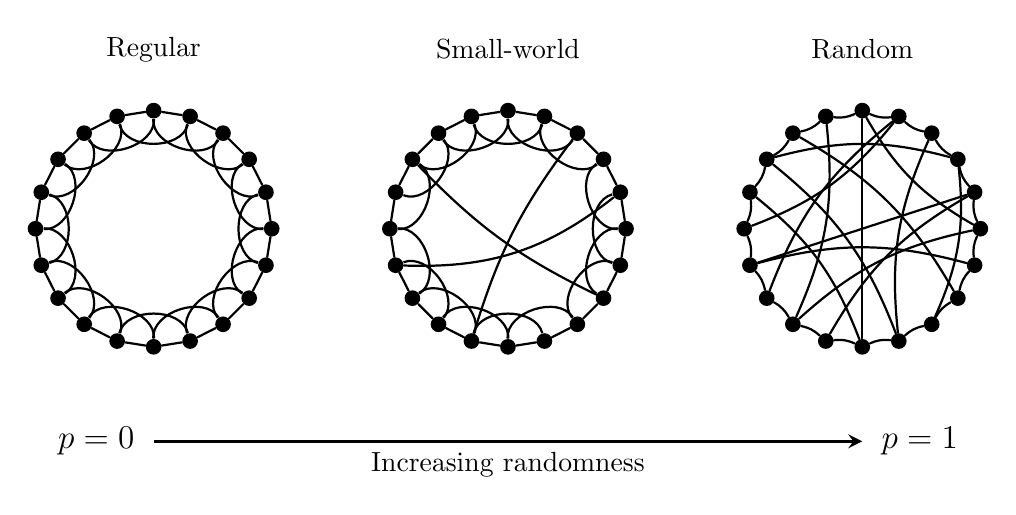
\begin{tikzpicture}[scale=0.6]
    % --- CONFIGURAZIONE ---
    \tikzset{
        node_style/.style={circle, fill=black, inner sep=2pt},
        edge_style/.style={thick, line cap=round},
        curved_edge/.style={thick, bend right=75} 
    }

    % Numero di nodi
    \def\N{20}
    % Raggio
    \def\R{2.5}

    % ===================================================
    % 1. REGULAR (Reticolo Regolare)
    % ===================================================
    \begin{scope}[xshift=0cm]
        \node[] at (0, 3.8) {Regular};
        
        \foreach \i in {1,...,\N} {
            \node[node_style] (n\i) at ({90 - 360/\N * (\i - 1)}:\R) {};
        }
        
        \foreach \i in {1,...,\N} {
            \pgfmathsetmacro{\next}{int(mod(\i, \N) + 1)}
            \pgfmathsetmacro{\nextnext}{int(mod(\i + 1, \N) + 1)}
            
            \draw[edge_style] (n\i) -- (n\next);
            \draw[curved_edge] (n\i) to (n\nextnext);
        }
    \end{scope}

    % ===================================================
    % 2. SMALL-WORLD (Piccolo Mondo)
    % ===================================================
    \begin{scope}[xshift=7.5cm]
        \node[] at (0, 3.8) {Small-world};
        
        \foreach \i in {1,...,\N} {
            \node[node_style] (m\i) at ({90 - 360/\N * (\i - 1)}:\R) {};
        }
        
        \foreach \i in {1,...,\N} {
            \pgfmathsetmacro{\next}{int(mod(\i, \N) + 1)}
            \pgfmathsetmacro{\nextnext}{int(mod(\i + 1, \N) + 1)}
            
            \draw[edge_style] (m\i) -- (m\next);
            
            % Rimuoviamo il collegamento uscente dai nodi 3, 8 e 15
            \ifnum \i=3 \else \ifnum \i=8 \else \ifnum \i=15 \else
                \draw[curved_edge] (m\i) to (m\nextnext);
            \fi\fi\fi
        }
        
        % Shortcuts
        \draw[edge_style] (m3) to[bend right=10] (m12); 
        \draw[edge_style] (m8) to[bend left=10] (m18);  
        \draw[edge_style] (m15) to[bend right=20] (m5); 
    \end{scope}

    % ===================================================
    % 3. RANDOM (Casuale)
    % ===================================================
    \begin{scope}[xshift=15cm]
        \node[] at (0, 3.8) {Random};
        
        % Creazione nodi r1...r20
        \foreach \i in {1,...,\N} {
            \node[node_style] (r\i) at ({90 - 360/\N * (\i - 1)}:\R) {};
        }
        
        % Lista degli archi compattata per evitare problemi di spazi
        \foreach \u/\v in {
            1/2, 2/3, 3/4, 4/5, 5/6, 6/7, 7/8, 8/9, 9/10,
            10/11, 11/12, 12/13, 13/14, 14/15, 15/16, 16/17, 17/18, 18/19, 19/20, 20/1,
            1/6, 2/14, 3/10, 4/18, 5/12, 7/15, 8/19, 9/4, 11/17, 13/20, 16/2, 6/13, 10/18%
        } {
            % FIX: eval(u) e eval(v) rimuovono eventuali spazi fantasma
            \pgfmathsetmacro{\U}{int(\u)}
            \pgfmathsetmacro{\V}{int(\v)}
            \draw[edge_style] (r\U) to[bend right=15] (r\V);
        }
        
        \draw[edge_style] (r1) to (r11);
        \draw[edge_style] (r5) to (r15);
    \end{scope}

    % ===================================================
    % BARRA INFERIORE
    % ===================================================
    \begin{scope}[yshift=-4.5cm]
        \draw[->, >=stealth, very thick] (0, 0) -- (15, 0);
        \node[font=\large, anchor=east] at (-0.2, 0) {$p=0$};
        \node[font=\large, anchor=west] at (15.2, 0) {$p=1$};
        \node[] at (7.5, -0.5) {Increasing randomness};
    \end{scope}

\end{tikzpicture}
\end{figure}

\hfill \\


La scoperta chiave è ciò che accade per valori intermedi di $p$:
\begin{itemize}
\item La lunghezza del cammino $L(p)$ cala \textit{molto velocemente} (logaritmicamente) non appena $p > 0$. Le prime poche "scorciatoie" riducono drasticamente il diametro.
\item Il clustering $C(p)$ cala \textit{lentamente} (linearmente) con $p$.
\end{itemize}
Questo modello mostra un ampio regime "small-world" ($p$ piccolo) dove $L(p)$ è piccolo (come un grafo casuale) ma $C(p)$ è alto (come un reticolo regolare), corrispondendo ai dati empirici di molte reti reali.


\hfill \\

\begin{figure}[htbp]
    \centering
    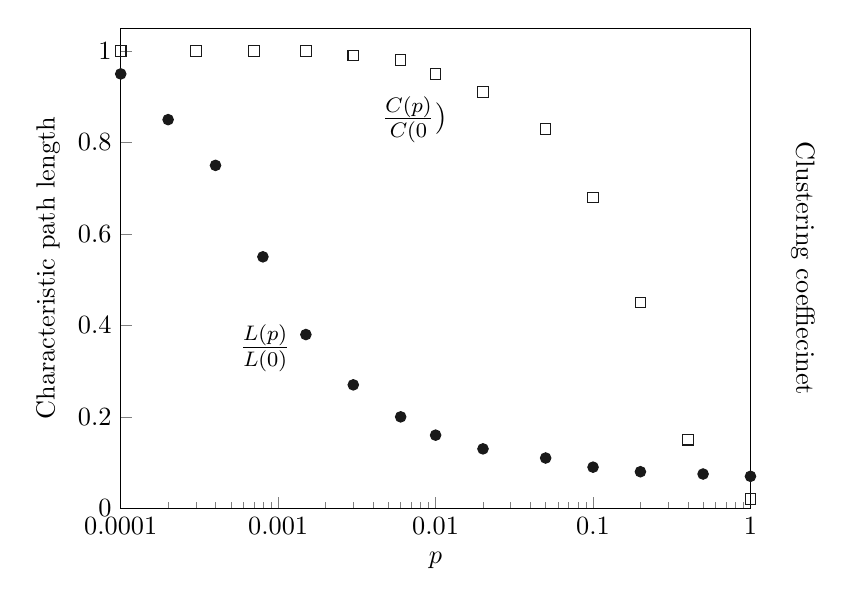
\begin{tikzpicture}[scale=0.95]
        \begin{semilogxaxis}[
            width=10cm, height=8cm,
            xmin=0.0001, xmax=1,
            ymin=0, ymax=1.05,
            xlabel={$p$},
            ylabel={Characteristic path length},
            % Rimuove i numeri sull'asse Y per metterli come nell'immagine o lascia standard
            ytick={0, 0.2, 0.4, 0.6, 0.8, 1.0},
            % Gestione dei tick dell'asse X (potenze di 10)
            xtick={0.0001, 0.001, 0.01, 0.1, 1},
            xticklabels={0.0001, 0.001, 0.01, 0.1, 1},
            % Permette di disegnare fuori dal grafico (per le annotazioni)
            clip=false,
            % Stile dei tick
            tick pos=left,
            tick align=inside,
            major tick length=0.15cm,
            minor tick length=0.08cm,
        ]

            % ==========================
            % SERIE DATI: L(p)/L(0) - Cerchi neri
            % ==========================
            \addplot[only marks, mark=*, mark size=2pt, color=black!90] coordinates {
                (0.0001, 0.95)
                (0.0002, 0.85)
                (0.0004, 0.75)
                (0.0008, 0.55)
                (0.0015, 0.38)
                (0.003, 0.27)
                (0.006, 0.20)
                (0.01, 0.16)
                (0.02, 0.13)
                (0.05, 0.11)
                (0.1, 0.09)
                (0.2, 0.08)
                (0.5, 0.075)
                (1.0, 0.07)
            };
            
            % Etichetta interna L(p)/L(0)
            \node[anchor=west] at (axis cs: 0.0005, 0.35) {\large $\frac{L(p)}{ L(0)}$};


            % ==========================
            % SERIE DATI: C(p)/C(0) - Quadrati vuoti
            % ==========================
            \addplot[only marks, mark=square, mark size=2pt, color=black!90] coordinates {
                (0.0001, 1.0)
                (0.0003, 1.0)
                (0.0007, 1.0)
                (0.0015, 1.0)
                (0.003, 0.99)
                (0.006, 0.98)
                (0.01, 0.95)
                (0.02, 0.91)
                (0.05, 0.83)
                (0.1, 0.68)
                (0.2, 0.45)
                (0.4, 0.15)
                (1.0, 0.02)
            };

            % Etichetta interna C(p)/C(0)
            \node[anchor=west] at (axis cs: 0.004, 0.85) {\large $\frac{C(p)}{ C(0})$};


            % ==========================
            % ANNOTAZIONE BLU (In alto)
            % ==========================
            % Nodo per il testo\node[align=left, font=\small, color=black] (blueText) at (axis cs: 0.05, 1.25) {C(p) remains almost constant at its value for the regular lattice, indicating\\ that the transition to a small world is almost undetectable at the local level. };
            % Linea blu sotto il testo \draw[blue, thick] (blueText.south west) -- (blueText.south east);
            % Freccia blu \draw[->, >=stealth, blue, thick] (blueText.south) -- (axis cs: 0.05, 0.85);


            % ==========================
            % ANNOTAZIONE ROSSA (In basso)
            % ==========================
            % Nodo per il testo \node[align=left, font=\small, color=black, anchor=north] (redText) at (axis cs: 0.004, -0.25) {Rapid drop in L(p), corresponding to the onset of the small-world phenomenon.};
            % Linea rossa sopra il testo\draw[red!80!orange, thick] (redText.north west) -- (redText.north east);
            % Freccia rossa \draw[->, >=stealth, red!80!orange, thick] (redText.north) -- (axis cs: 0.002, 0.25);


            % ==========================
            % ETICHETTA ASSE DESTRO
            % ==========================
            \node[rotate=-90, anchor=south] at (rel axis cs: 1.05, 0.5) {Clustering coeffiecinet};

        \end{semilogxaxis}
    \end{tikzpicture}
    \caption{Il grafico mostra la lunghezza del cammino caratteristica normalizzata $L(p)/L(0)$ e il coefficiente di clustering normalizzato $C(p)/C(0)$ in funzione della probabilità di ri-cablaggio $p$. Si nota un ampio intervallo di $p$ dove la rete mantiene un alto clustering (tipico dei reticoli regolari) ma acquisisce una bassa lunghezza di cammino (tipica dei grafi casuali).}
    \label{fig:watts_strogatz_chart}
\end{figure}

\newpage
\section{Modelli di Rete IV: Modello Barabási-Albert}
Questo modello (1999) introduce un concetto diverso: la rete non è statica ma \textbf{cresce} nel tempo. Ha due ingredienti chiave:

\begin{enumerate}
\item \textbf{Crescita:} Si inizia con un piccolo insieme di $n_0$ nodi. Ad ogni passo temporale, si aggiunge un nuovo nodo al sistema.
\item \textbf{Attaccamento Preferenziale:} Il nuovo nodo si connette a $m_0$ nodi esistenti. La probabilità $\mathbb{P}(k_i)$ di connettersi a un nodo esistente $i$ non è uniforme; è proporzionale al grado attuale di quel nodo $k_i$.
\end{enumerate}
\begin{tcolorbox}[colback=yellow!25, colframe=yellow!75!orange, coltitle=black, title=\textbf{Regola dell'Attaccamento Preferenziale}]
\begin{equation} \label{eq:ba}
\mathbb{P}(k_i) = \frac{k_i}{\sum_j k_j}
\end{equation}
\end{tcolorbox}

Questo meccanismo rich get richer implica che i nodi che sono già altamente connessi hanno maggiori probabilità di ottenere nuove connessioni. Questo modello genera naturalmente una distribuzione di grado a legge di potenza (che risolveremo nella prossima lezione) e, per definizione, crea una singola componente gigante ($S=1$).

